% Evaluation
\section{Evaluation}
\label{Evaluation}

We implemented Alano in C++ and evaluated the algorithms in a cluster of 9 servers, each equipped with an Intel Xeon 2.6GHz CPU with 24 hyper-threading cores, 64GB memory and 1T SSD. The basic settings in the evaluation are: 


$N=1000$, $t_0=20ms$, $p_n=0.5$, $\delta=1000$ slots. That is, the network is composed of $1000$ nodes, $0.5$ density, and maximum start time offset $1000$ slots, where each slot is $20 ms$. 

These settings make the network more complicated and realistic than that in \cite{Kandhalu2010, Sun2014b, Qiu2016, Chen2015, Bakht2012, McGlynn2001, Vasudevan2009, Jiang2005, Dutta2008, You2011, Song2014}.

We evaluated discovery latency of Alano, Aloha-like~\cite{You2011}, Hello~\cite{Sun2014b}, Hedis~\cite{}, and Searchlight~\cite{} in partially-connected network. 

\subsection{Comparison of Discovery Latency}

\begin{figure}[!t]
\centering
\subfigure[Uniform Distribution]{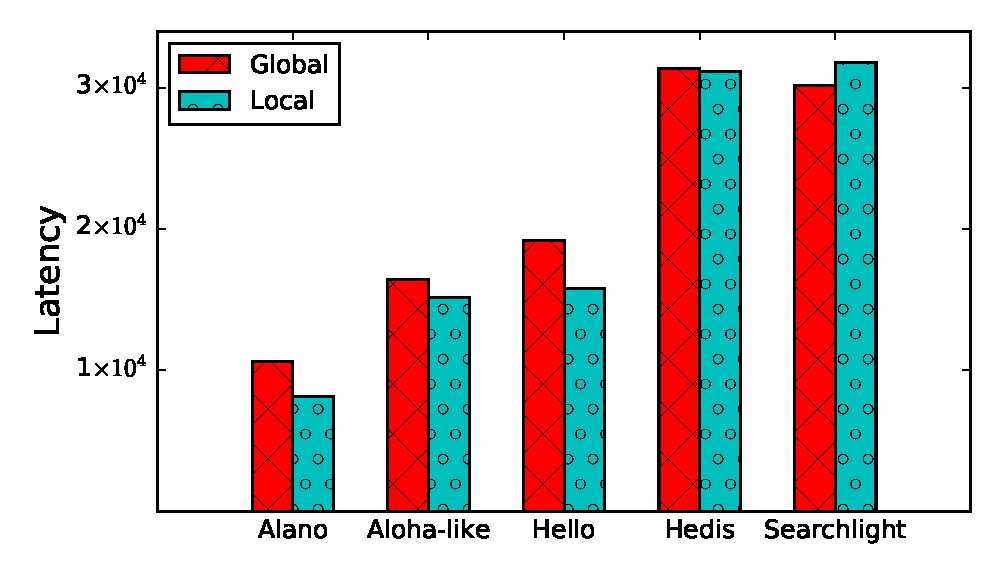
\includegraphics[width=1.65in]{Figure/latency_uniform}}
\hspace{0.01in}
\subfigure[Normal Distribution]{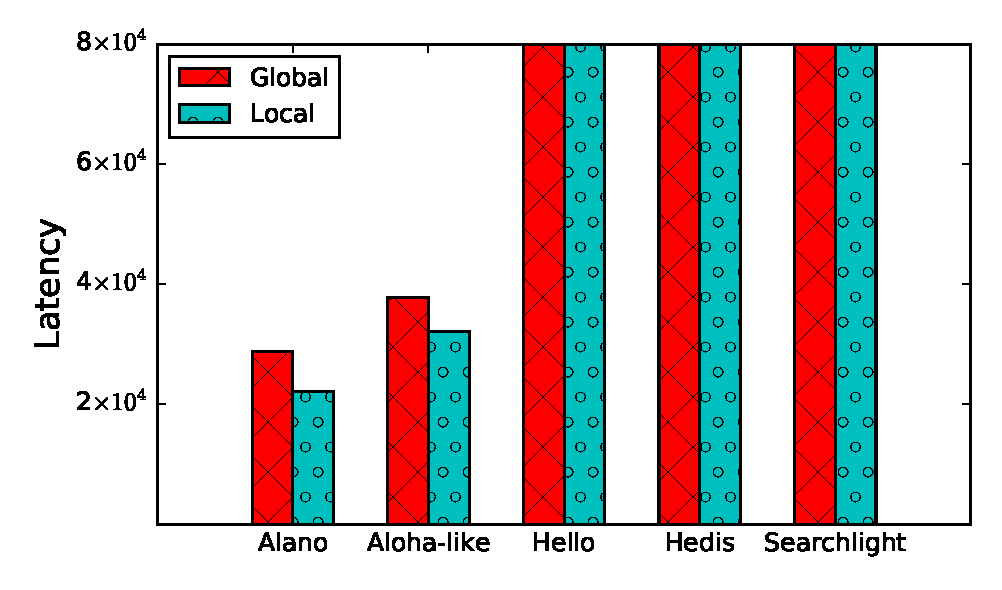
\includegraphics[width=1.65in]{Figure/latency_normal}}
\caption{Panacea-WCD achieves higher discovery rate with CD.}
\label{fig_timerate}
\end{figure}

\subsection{Comparison of Discovery Rate}

\begin{figure}[!t]
\centering
\subfigure[Synchronous Scenario]{\includegraphics[width=1.65in]{figure/time_rate_syn}}
\hspace{0.01in}
\subfigure[Asynchronous Scenario]{\includegraphics[width=1.65in]{figure/time_rate_asyn}}
\caption{Panacea-WCD achieves higher discovery rate with CD.}
\label{fig_timerate}
\end{figure}


